\documentclass[lettersize,journal]{IEEEtran}
\usepackage{amsmath,amsfonts}
\usepackage{algorithmicx, algorithm, algpseudocode}
\usepackage{array}
%\usepackage[caption=false,font=normalsize,labelfont=sf,textfont=sf]{subfig}
\usepackage[font=small]{caption}
\usepackage[labelformat=simple,font=scriptsize]{subcaption}
\renewcommand\thesubfigure{(\alph{subfigure})}
%\usepackage{textcomp}
%\usepackage{stfloats}
\usepackage{adjustbox}
\usepackage{url}
\usepackage{verbatim}
\usepackage{graphicx}
\usepackage{cite}
% updated with editorial comments 8/9/2021

\begin{document}

\title{Covert Communication in \\Autoencoder Wireless Systems}

\author{Ali~Mohamamdi~Teshnizi,~\IEEEmembership{Student Member,~IEEE,}
	Majid~Ghaderi,~\IEEEmembership{Member,~IEEE,}
	and~Dennis~Goeckel,~\IEEEmembership{Fellow,~IEEE}% <-this % stops a space
}

% The paper headers
\markboth{Journal of Cognitive Communications and Networking,~Vol.~9, No.~3, June~2023}%
{Shell \MakeLowercase{\textit{et al.}}: A Sample Article Using IEEEtran.cls for IEEE Journals}

%\IEEEpubid{0000--0000/00\$00.00~\copyright~2021 IEEE}
% Remember, if you use this you must call \IEEEpubidadjcol in the second
% column for its text to clear the IEEEpubid mark.

\maketitle

\begin{abstract}
Hiding the wireless communication by transmitter Alice to intended receiver Bob from a capable and attentive adversary Willie has been widely studied under the moniker ``covert communications''.  However, when such covert communication is done in the presence of allowable system communications, there has been little study of both hiding the signal and preserving the performance of those allowable communications. Here, by treating Alice, Bob, and Willie as a generator, decoder, and discriminator neural network, we perform joint training in an adversarial setting to yield a covert communication scheme that can be added to any normal autoencoder. The method does not depend on the characteristics of the cover signal or the type of channel and it is developed for both single-user and multi-user systems. Numerical results indicate that we are able to establish a reliable undetectable channel between Alice and Bob, regardless of the cover signal or type of fading, and that the signal causes almost no disturbance to the ongoing normal operation of the system.
\end{abstract}

\begin{comment}
	Covert communication, wireless communication, autoencoder wireless systems
\end{comment}
\section{Introduction}
\label{s:intro}

Due to the shared and broadcast nature of wireless channels, there is considerable attention on the security and privacy aspects of wireless communications. While traditional cryptography methods and physical-layer securities can protect the confidentiality of the content (i.e the information transmitted over the channel), there are occasions that hiding the very existence of the communication channel is more vital than securing the communicated message itself. Examples of such situations are military operations, cyber-espionage, social unrest, or communication parties' privacy. All above have motivated the study of hidden communication channels, namely, "covert channels" \cite{lampson1973note}.\\
The preliminary attempt to obtain covertness started with the study of spread spectrum, which began almost a century ago with the main purpose of hiding military communications. The idea is to spread the transmit power into the noise so that the communication stays hidden. Many works continued to further examine different aspects of this idea, yet the fundamental performance limits of such work were unknown until recently when Bash et al. \cite{bash2012square} established a square root limit on the number of covert bits that can be reliably sent over an additive white Gaussian noise (AWGN) channel while remaining covert to a channel's observer. Followed by this work, there has been a surge of interest in examining covert channels \cite{sobers2017covert,soltani2018covert} especially in point-to-point wireless communication models.\\
In the last decade, majority of the research works on covert communication focus on integration of covert communication techniques into the current and future wireless technologies, such as 6G wireless networks and IoT. With the advent of AI and recent advances in computer's computation power and algorithmic designs, machine learning (ML) is now becoming an integral part of many research topics. Correspondingly, wireless community started to adopt machine learning techniques and use them as solutions to the various network optimization problems, which were traditionally handled with statistical models. Deep neural networks (DNNs) in particular, a major force in machine learning, are now applied into many of these tasks including signal classification, channel estimation, transmitter identification, jamming and anti-jamming [?].\\
More recently, as a replacement for conventional modular-based designs, an end-to-end communication model based on deep learning methods has emerged \cite{o2017introduction}. In this new paradigm, the transmitter and receiver are jointly trained as the encoder and decoder of an autoencoder network. While the transmitter learns to encode the transmitted symbol to an embedding vector of wireless signals, the decoder, on the other side, learns to retrieve that symbol back from the transmitted signal after passing through the channel. One noticeable difference between end-to-end systems and conventional modular designs is that in end-to-end systems, the encoder learns coding and modulation tasks simultaneously as opposed to having separate modules to perform each task. This is also true for the decoder of the system that jointly learns demodulation and decoding. Given the fact that channel distortions usually have a non-linear behavior, a DNN-based communication model is expected to capture these dissimilitudes better compared to a statistical model. That means, these systems can learn more complex channel effects and can operate more robustly under different noise levels and channel imperfections \cite{wang2017deep}.
In this work, we introduce a novel deep learning based covert communication method inspired by steganography techniques using generative adversarial networks (GANs). The proposed covert scheme is designed for the next generation autoencoder-based wireless communication models, which are believed to be replacing traditional modular based wireless systems in the near future. However, there is no limitation on integrating our covert model to the current wireless communication systems.\\
The contributions of this work can be expressed as:
\begin{enumerate}
	\item We propose a novel covert communication method using GANs that works independent of the channel and cover signals of the wireless system.
	\item We train and evaluate our system on two different channel models of AWGN and Rayleigh fading to be more compliant to a realistic wireless communication model.
	\item We also measured both the performance of our covert model and the normal autoencoder-based communication system in terms of error rates to comprehend effectiveness of covert scheme and the impact of it on the existing communication between normal users.
\end{enumerate}

\section{Related Works}
\label{s:related}
Since the main idea of our work stems from the stenography techniques, we first briefly go over the history and the current state of this field of research. We then continue this section reviewing some of the existing approaches of establishing covert communication at the physical layer of wireless networks.


\textbf{Image Steganography}: Deep learning algorithms have proven their efficiency in many aspects. Steganography is one of these areas that has benefited tremendously from deep learning advancements in recent years. Convolution neural networks (CNNs) for instance, which are generally used in computer vision tasks, have shown outstanding results in image steganalysis \cite{tan2014stacked,qian2015deep,xu2016structural}, replacing the traditional statistical methods. One of the earliest works of image steganography using deep neural networks is a work by \cite{baluja2017hiding}. In this work, Baluja proposes a hiding scheme in which the three networks of preparation, hiding, and reveal sort out the secret encoding and decoding task. The preparation network transforms the hidden message into features that are commonly used for compressing images. Then, the hiding network embeds it into the cover image and sends it to the reveal network, where the secret message gets extracted from the container image. Following this work, it was discovered that the existence of preparation network is not necessary and the framework can be expressed in a simpler form by excluding this network \cite{zhang2021brief}. The disadvantage of these schemes is that the encoding process is reliant on the cover image. To address this, Zhang et al. \cite{zhang2020udh} propose a new architecture in which secret message can be encoded independent of the cover image. Beside having more flexibility on hiding the information, this approach has also become an effective method for image watermarking. To manifest robustness against steganalysis practices, researchers started to adopt generative adversarial network (GAN) architectures \cite{goodfellow2014generative}. Volkhonskiy et al. \cite{volkhonskiy2020steganographic} propose one of the first steganography techniques based on GAN networks. The main idea of their work is to use a generative network to produce a new set of cover images that when carries the secret message using any of the available steganography techniques will be less exposed to be detected by a discriminator network (i.e. a steganalysis network). Similarly, Hayes et al. \cite{hayes2017generating} introduce a GAN-based steganography technique with a different objective for the generator network. Instead of generating cover images, the generator learns to embed secret messages into the cover images so that the discriminator cannot distinguish cover images from stenographic images. Although this adversarial scenario was preliminary introduced for hiding data in images, researchers found it so versatile that it has been applied into the other forms of data such as video, audio and text. This has inspired us to investigate the applicability of such techniques in wireless signals domain.


\textbf{Covert Communication}: Covert communication has been applied to almost every network layer and protocol, such as IP \cite{cabuk2004ip}, MAC \cite{sheikholeslami2020covert}, and DNS \cite{nussbaum2009robust}. However, covert communication at the physical layer has not been receiving much attention until recently. Dutta et al. \cite{dutta2012secret} are on of the first researchers who developed a covert communication technique for the physical layer of the wireless communication systems. They leverage the communication noise, which can be caused either by the channel or the hardware imperfections, as a mean to establish the covert channel. In their method, messages are covertly encoded in the constellation error of the normal cover signals. Similarly, Cao et al. \cite{cao2018wireless} further improved this method with the goal of reducing probability of detection. However, distortions that these methods cause in the statistical properties of the system were later found not so difficult to be detected using steganalysis methods \cite{huang2020exploiting}, which in turn results in compromising the channel. More recent works have explored the viability of deep neural networks in covert communication problem. Sankhe et al. \cite{sankhe2019impairment} propose a method called Impairment Shift Keying that produces subtle variations in normal signals in a controlled way such that a CNN model can be trained to classify them as zeros or ones. Although the impact of their covert method on the system's communication error rate is as small as 1\%,  authors in \cite{huang2021detection} showed that even tiny modifications to the signals' constellation points can be detected using a CNN model trained on the amplitude and phase characteristics of the error vector magnitude (EVM) and constellation points. Besides, their scheme relies on existing hardware impairments in the system, which is not the case in many deployments. To find an optimal solution for the highest covert rate and minimum probability of detection, Liao et al. \cite{liao2020generative} employed a GAN model that can adaptively adjust the signal power at a relay station for establishing a covert communication. This requires the covert users to have access to a cooperative relay node that is not the case in many communication scenarios. Another example of adversarial training for covert communication can be found in \cite{kim2022covert}. Their setup contains a transmitter communicating with a receiver through a Reconfigurable Intelligent Surface (RIS), and their goal is to keep this communication covert from a prospective eavesdropper. Both the intended receiver and the eavesdropper use CNN classifiers to detect the signals. This scenario raises the same concern of the previous work's that is the necessity of existence of a relay node in the deployment. Moreover, perturbations added to the signals to deceive the eavesdropper are crafted using fast gradient method (FGM) \cite{goodfellow2014explaining}, which in \cite{bahramali2021robust} was shown easy to counter using the existing countermeasure techniques. Our work differs from these two works in two aspects. First, our proposed method relies on no external entities or external factors, such as relay nodes and hardware impairments, and this helps with the generality of our model. Second, we use a generative network to produce a set of perturbations to maximize the robustness of our attacks against the system's observer or eavesdropper. 

One of the most related works to ours is the covert scheme proposed by Mohammed et al. \cite{mohammed2021adversarial}. They formulate the covert communication as a three-player game in which networks compete in an adversarial setting to obtain the optimal solution. In their setup, the encoder and decoder networks learn to covertly communicate through a form of noise and simultaneously try to confuse a detector network that tries to tell whether the users are covertly communicating or it is just the normal transmissions going through. While our proposed method shares some of the ideas of aforementioned work, there are a couple of limitations in this work that ours aims to address. First, our model is not leveraging on any hardware impairment noise and embeds the covert signals into the existing channel's noise. Second, in the previous work, the impact of added covert signals on communication is unknown, but our model is optimized to preserve the performance of normal communication. And finally, previous work assumes the channel between users to be AWGN, however, this is not an accurate model for simulating the channel effects in wireless communications due to fading. Our work addresses this by proposing a robust method against different channel models including Rayleigh and Rician fading channels.
\section{Background On Autoencoder Communication Systems}
\label{s:design}
An autoencoder-based communication system is an end-to-end learning paradigm that abstracts out the coding and modulation components of a  traditional modular communication system by replacing the transmitter and receiver with DNNs. You can see a block diagram of such a system in figure ?. The encoder (transmitter) first uses a mapping to transform \(k\) bits of data into a message \(s\) where \(s \in \{1,...,M\}\) and \(M = 2^k\). Then it takes this transformed message as an input and generates a signal \(x = E(s) \in \mathbb{R}^{2n}\), which is a real valued vector. This \(2 \times n\) dimensional real valued vector can be treated as an \(n\) dimensional complex vector where \(n\) is the number of channel uses the signal needs to be transmitted over. Then, the channel effect \(z\), which is usually considered to be AWGN, is added to the signal vector. Thus, the received signal at the receiver carries within iselfs noise of the channel and can be expressed as \(y = x + z\). The decoder (receiver) applies the transformation \(g: \mathbb{R}^{2n} \rightarrow M \) to outputs the reconstructed version of the message \(s\), which is denoted as \(\hat{s} = g(y)\).
\section{Our Covert Communication System Model}
\label{s:model}
In this section, we begin with an overview of our covert communication model and will further discuss the details of our scheme in the subsequent sections.
\subsection{Overview}
An overview of our system architecture is shown in figure (\ref{fig:system_architecture}). The main idea of our work is to establish a covert channel on top of a normal communication between a sender (UserTX) and a receiver (UserRX) who are using an autoencoder-based wireless system to communicate. We consider both an AWGN and a Rayleigh fading channels between our communication parties. The objective of the covert sender (Alice) is to secretly communicate with the covert receiver (Bob) by embedding her messages in form of perturbations that have similar statistical properties as of the channel's noise. This is achieved by help of an observer (Willie), which acts as an observer of the channel, trying to rigorously classify transmitted signals as covert and non-covert after they pass through the channel.\\
\subsection{System Architecture}
As mentioned above, there are three main actors in our covert system which we call them by their placeholder names: Alice, Bob, and Willie from now on. All three are collaborating in our covert scheme and are represented by DNNs. Alice is using a generative model that embeds a confidential message \(m\) into a covert noise vector \(\hat{z}\). This covert signal is then transmitted over the channel after being added to a normal signal \(x\). Similar to every covert communication scheme, there is an observer or warden in the system that will be alerted when seeing any deviation in the statistical properties of the channel. To this end, we are implicitly incorporating a statistical undetectability constraint on the produced covert signals by having a discriminator network employed by Willie. The presence of this discriminator network helps us to ensure that these added covert noise signals are distributed as the real channel noise, making them undetectable. Mathematically, in the AWGN channel model, it means \(\hat{z} \sim \mathcal{CN}(0, \sigma_{chl}^2)\) where \(\sigma_{chl}^2\) will be the variance of the channel's noise.\\
For a given binary secret message \(m\), Alice first one-hot encodes the message and then uses its generator model to produce a covert noise signal \(\hat{z}\). This covert signal is then added to a vector of a normal signal, which is carrying messages between UserTX and UserRX. Therefore, the covert signals before being transmitted over the channel can be denoted as:
\begin{equation}
	\hat{x} = x + \hat{z}
\end{equation}
The signal is then transmitted over the channel. We mentioned that we assume the channel between sender and receiver of the system to be AWGN or Rayleigh. Therefore, there will be two different channel outputs for these two different channel models that can be represented as a mapping function \(C(\cdot)\):
\subsubsection{AWGN Channel Output}
For the AWGN channel model, the signal received at the receiver carries within itself the channel noise effect \(z \sim \mathcal{N}(0, \sigma_{chl}^2)\). Thus, the channel function \(C(\cdot)\) and final covert signal \(\hat{y}\) can be represented as:
\begin{equation}
	C(\hat{x}) \Rightarrow \hat{y} = \hat{x} + z
\end{equation}
\subsubsection{Rayleigh Fading Channel Output}
For the Rayleigh fading channel model, we consider a flat block fading channel where each codeword is assumed to be faded independently. Let \(h\) be the fading coefficient when transmitting the codeword \(\hat{x}\), then the channel function \(C(.)\) and and the final covert signal \(\hat{y}\) is given by:
\begin{equation}
	C(\hat{x}) \Rightarrow \hat{y} = h \cdot \hat{x} + z
\end{equation}
On the receiver side, Bob receives a transmitted signal \(\hat{y}\) after the channel noise is added into it. He uses its decoder network to reconstruct the covert message \(\hat{m}\). Meanwhile, the UserRX is using the same signal to extract the normal message \(\hat{s}\), which is the reconstructed message of \(s\) sent from UserTX. The statistical properties of the signals on the channel are captured by Willie who observes the channel continuously. His objective is to classify sequences of normal \(y\) and covert signals \(\hat{y}\) passed through the channel and provide useful feedback to Alice. This feedback helps Alice to modify the produced covert signals such that they are indistinguishable from the normal signals of the communication. In other words, it ensures that both normal and covert signals have the same statistical properties.
\subsection{General Formulation}
The very first objective of our covert model is to have a working covert channel. To this end, Bob has to have a plausible accuracy in decoding covert messages that Alice sends through the covert signals \(\hat{y}\). As mentioned in previous section, Alice employs a generative model instead of an encoder model suggested by \cite{mohammed2021adversarial}. Using an encoder model to produce covert signal perturbations will map each covert message \(m\) to a single covert noise vector \(\hat{z}\). Inevitably, these deterministic covert perturbations can be eliminated with ease by a careful observer or defender as it was shown in the work of Bahramali et al. \cite{bahramali2021robust}, who studied the covert attack problem against autoencoder wireless networks. Thus, we use an stochastic generative model for Alice so that each covert message maps to a set of different covert noise signals. Let \(A(\cdot)\) be the underlying function of Alice's generative model that takes a random trigger \(t \sim \mathcal{N}(0, 1)\) and a covert message \(m\)) and produces a covert signal \(\hat{z}\)) (we denote the corresponding covert signal as \(\hat{z}_{m, t} = A(m, t)\)). Let also  \(B(\cdot)\) be the underlying function of the decoder network that Bob makes use of to reconstruct the covert message \(\hat{m}\). Then the reliability of communication between Alice and Bob is achieved using the below loss function:
\begin{equation}
	\begin{array}{l} \label{bob_loss}
	\mathcal{L}_{Bob} = \mathbb{E}_{m}[CE(\hat{m}, m)] \\ \Rightarrow \mathbb{E}_{m}[CE(B(C(A(m, t) + x)), m)]
	\end{array}
\end{equation}
where \(CE(\cdot)\) is the cross entropy between the reconstructed covert message \(\hat{m}\) and the actual covert message \(m\). This equation can be used to optimize both for Alice's and Bob's networks by freezing one or the other network's parameters iteratively. While (\ref{bob_loss}) ensures the communication accuracy, we also need to bear in mind that the generated perturbations should have no detrimental impact on the normal communication between UserTX and UserRX, otherwise an unexpected high error rate in the communication can be an indication for an abnormal behavior. We apply this constraint by optimizing for the below loss function during training Alice's generator network:
\begin{equation}
	\begin{array}{l} \label{alice_user_loss}
	\mathcal{L}_{UserRX} = \mathbb{E}_{m}[CE(\hat{s}, s)] \\ \Rightarrow \mathbb{E}_{m}[CE(D(C(A(m, t) + E(s))), s)]
	\end{array}
\end{equation}
where \(D(\cdot)\) is UserRX's decoder network function, and \(E(\cdot)\) is the underlying function of the UserTX's encoder network. Note that both UserTX's encoder and UserRX's decoder networks are frozen during this training and only Alice's parameters are updated.\\
In our model, the observer entity or Willie, acts as the discriminator in GAN models \cite{goodfellow2014generative}. The so-called real and fake data in GANs' discriminator training here is mapped to non-covert and covert signals and we define the loss function as:
\begin{equation}
		\begin{array}{l} \label{willie_loss}
	\mathcal{L}_{Willie} = \mathbb{E}_{m}[BCE(\hat{y}, y)] \\ \Rightarrow \mathbb{E}_{m}[BCE(C(A(m,t) + x), C(x))]
	\end{array}
\end{equation}
where \(BCE(\cdot)\) is the binary cross entropy between the covert signal \(\hat{y}\) and the normal signal \(y\). This adversarial training against Alice network ensures that Willie will be adequately trained to tell covert and non-covert signals apart. On the other hand, we mentioned that the covert signals that Alice produces should not deviate from the statistical properties of the normal signals on the channel, otherwise the observer of the channel can detect and mitigate the covert communication. To achieve this undetectability property, we pose a new constraint on Alice's optimization function for maximizing Willie's uncertainty about the covert predictions. Having a regularizer as such helps Alice and Bob to form their covert communication in way that is indistinguishable from the actual channel's noise, yet understandable by both. Altogether, Alice's loss function can be expressed as a weighted sum of three different objectives:
\begin{equation}
	\begin{array}{l} \label{alice_loss}
	\mathcal{L}_{Alice} = \lambda_{Bob} \mathcal{L}_{Bob} + \lambda_{UserRX} \mathcal{L}_{UserRX} - \lambda_{Willie} \mathcal{L}_{Willie}
\end{array}
\end{equation}
where \(\lambda_{Bob}\), \(\lambda_{UserRX}\), and \(\lambda_{Willie}\) determine the importance of each objective for training Alice.
\iffalse Algorithm (?) summarizes our approach for optimizing the whole system. \fi
\subsection{Neural Network Architecture}
Before discussing the architecture of our neural network models, we need to state that the communication between UserTX and UserRX is taking place using an autoencoder communication model, which is utilized to encode and decode the normal messages. Since the focus of this work is not to introduce an autoencoder wireless network, we briefly explain how this model works. Also, an overview of the implemented autoencoder model's network architecture can be found in table (?). A more detailed explanation of such a network and the training procedure can be found in the original paper \cite{o2017introduction}. The other three entities of our scheme, which are our covert actors, also use neural networks to function. A detailed network architecture of each is likewise represented in table (?).\\
\begin{figure}[tp]
	\center
	\begin{subfigure}{0.35\textwidth}
		\includegraphics[width=\linewidth]{figs/autoencoder_bler_awgn}
		\caption{AWGN channel}
	\end{subfigure}
	\begin{subfigure}{0.35\textwidth}
		\includegraphics[width=\linewidth]{figs/autoencoder_bler_rayleigh}
		\caption{Rayleigh fading channel}	
	\end{subfigure}
	\caption{Trained Autoencoder's BLER over a range of SNR values}
	\label{fig:autoencoder_bler}
\end{figure}
Similar to what is proposed in the original autoencoder wireless communication paper, our autoencoder model accepts a binary message \(s\) of size \(k\) bits. Afterwards, the encoder part first one-hot encodes the message to represent each message as a different class and then maps it to a vector of signals of size \(2 \times n\), where \(n\) is the number of channel uses. This transmitted signal is then given to a mapping function that applies the channel effects into it. On the receiver side, there will be two different structures given what the channel model is. In case of an AWGN channel model, the signal is simply passed through the decoder network and the intended message gets extracted. For the Rayleigh fading channel model, however, there will be a parameter estimation model that takes in the signal before it passes through the decoder network in order to estimate the channel's fading coefficients. Followed by this operation, the extracted signal along with the estimated parameters are passed to a transformation function that reverts the channel effects. In our case, we are using a simple division transformation function that divides the received signal by the estimated channel fading coefficients. Note that more complex transformation functions can be used and are described in \cite{o2017introduction}, however optimizing the performance of autoencoder model is out of the scope of this article. Eventually, the transformed signal is fed to the decoder's network and the original normal message is reconstructed by classifying the signal. Similar to the encoder network, Alice takes a covert message \(m\) and transforms it to its corresponding one-hot encoding representation so that each message belongs to a unique class. Next, given a random trigger \(t\), Alice uses its generator model to produce a covert noise signal \(\hat{z}\) and adds it to the normal signal \(x\) that is being transmitted at the time. Bob receives this covert signal that has undergone the channel's effects and feeds it through its decoder network regardless of what the channel model is and extracts the secret message by classifying the signal. Meanwhile, Willie receives the same covert signal \(\hat{y}\) and the non-covert signal \(y\) and outputs a confidence probability \(P\) on how probable it is for the signal to be normal.
For the Alice's generator model, we use multiple dense layers with ReLU and Tanh activation functions. The first layer of this model takes a trigger number \(t\) and an one-hot encoded covert message \(m\), and acts as embedding layer by enlarging the input's domain space. The following fully contacted layers are to extract the useful features and do the encoding process. The last layer of this model does a dimension transformation so that the generated covert signal \(\hat{z}\) complies with the dimension of the normal signal \(x\) on the channel. Bob's network has a more complicated structure as it has to decode the secret message from a signal \(\hat{y}\) that has been distorted stiffly as a result of the channel's effect. The received message by Bob first goes through the first layer of the network, which is a dense layer with a Tanh activation function, acting as a denoising layer. Then the data is passed through multiple 1-Dimensional Convolutional (1D Conv) layers that supposedly learn the coding that Alice has fabricated to encode the covert messages. We have found that using 1D Conv layers helps Bob and Alice achieving a better consistency in the accuracy of their communication, especially when the channel model is more complicated (i.e. when there is also fading in the channel). The rest of Bob's decoder network consists of two dense layers that does a domain remapping from the learned feature space to the covert message domain space. Similar to the UserRX's decoder network, Bob eventually predicts the covert message by doing a classification on the received signal.



\section{Experiments and Evaluation}
\label{s:eval}
Our experiments are divided into two sections. In the first section, we evaluate the performance of our trained autoencoder wireless networks. Note that is no covert communication in the these experiments, and the purpose is to tune the parameters of the autoencoder models and confirm their accurate performance and behavior in fading environments, in addition to the AWGN channels that is considered in the literature. In the next section, we discuss the performance of our implemented covert models in both single-user and multi-user cases in terms of their robustness to different channel models, data rates, and numbers of users.

\subsection{Base Single-User Autoencoder's Performance}
\textbf{Methodology}: We implemented an autoencoder communication network for normal communication between UserRX and UserTX. An autoencoder \(Autoencoder (n, k)\) is a neural network communication model that sends \(k\) bits of data in \(n\) channel uses. To make our results comparable with the original paper \cite{o2017introduction}, we chose our default parameters to be 8 and 4 for the number of channel uses and binary message size, respectively. However, we also evaluated our models for two other sets of parameters with the same data rate but different numbers of channel uses. This allowed us to examine how increasing the number of channel uses, or signal dimensionality, would affect communication performance. To train our autoencoder model, we generated two datasets for training and testing by randomly generating binary messages \(s\) of size \(k\). Specifically, we used 8192 random binary messages in the training set and 51200 random binary messages in the test set. We created a much larger dataset for testing to ensure that each signal \(X\) undergoes various channel distortions, providing a more accurate evaluation of the model's performance. We set the learning rate to 0.001 and optimized the model using the Adam optimizer \cite{kingma2014adam}. We used a batch size of 1024 and trained the model for 100 epochs. For the channel configuration, \textbf{we fixed the SNR value during training but evaluated the model's performance over a range of SNRs}. The SNR value for the AWGN channel was set to 4dB, while the values for the Rayleigh and Rician fading channels were 16dB. We chose these SNR values experimentally by training the models on different SNR values and identifying the value on which the model performed best.

\begin{figure*}[!tp]
	\center
	\begin{subfigure}{0.28\linewidth}
		\includegraphics[width=\linewidth]{figs/multi_autoencoder_bler_awgn}
		\caption{AWGN channel}
	\end{subfigure}
	\begin{subfigure}{0.28\linewidth}
		\includegraphics[width=\linewidth]{figs/multi_autoencoder_bler_rician}
		\caption{Rician fading channel}	
	\end{subfigure}
	\begin{subfigure}{0.28\linewidth}
		\includegraphics[width=\linewidth]{figs/multi_autoencoder_bler_rayleigh}
		\caption{Rayleigh fading channel}	
	\end{subfigure}
	\caption{The block error rates (BLERs) of our trained autoencoders compared with simulated results for different numbers of users over a range of SNR values in our multi-user case.}
	\label{fig:multi_autoencoder_bler}
\end{figure*}

\textbf{Results}: Fig. \ref{fig:autoencoder_bler} shows the block error rate (BLER) performance of our trained autoencoder communication models for various sets of parameters across a range of SNR values. The models were trained individually on AWGN, Rayleigh, and Rician fading channels and tested on the same channel they were trained on.
The plot reveals that despite having the same data and coding rate, increasing the signal dimension slightly enhances the performance of the autoencoder models. This phenomenon was first identified in \cite{o2017introduction}, which demonstrated that autoencoders trained over an AWGN channel can achieve a coding gain by learning a joint coding and modulation scheme. Our results support this finding and suggest that this behavior holds true for autoencoders trained on other channel models as well. However, it should be noted that a comprehensive study of the performance of autoencoder wireless systems for multiple channel types and parameters (n, k) goes beyond the scope of this work and is not the primary focus of this research.


\subsection{Base Multi-User Autoencoders' Performance}
\textbf{Methodology}: In the multi-user case, we have chosen the number of channel uses and the binary message size to be 8 and 4, respectively, as these are our default parameters. There are two reasons for selecting these parameters in this way. First, it allows us to compare our results with those obtained in \cite{o2017introduction}. Second, by having each user communicate at half the rate of BPSK, the results of our 2-user system are roughly comparable to a single-user system at the BPSK rate, while the 4-user system is comparable to a single-user system at the QPSK rate. To generate training and testing sets, we followed the same procedure outlined in the previous section. The remaining parameters, such as learning rate, number of epochs, batch size, and optimization algorithm, are kept the same as in the single-user system. For the channel configuration, we have chosen SNR values of 8dB for the AWGN channel, 16dB for the Rayleigh channel, and 14dB for the Rician channel during training. However, we evaluate our models over a range of SNR values.

\textbf{Results}: The performance of our trained autoencoder-based communication models in terms of block error rate (BLER) for a range of SNR values for different numbers of users is shown in Fig. \ref{fig:multi_autoencoder_bler}. In all charts, the 2-user and 4-user performances are depicted with blue and red colors, respectively, and the results are compared with simulated traditional BPSK and QPSK systems with hard decision decoding.
The results indicate that multi-user autoencoder models can achieve almost similar performance to their counterparts in the single-user cases when compared data rate-wise. However, we have also observed that while the AWGN and Rician autoencoders outperform their peers, the Rayleigh fading autoencoders do not. We attribute this to the more complex equalization task that the receiver in multi-user cases needs to undertake. This becomes more evident when we compare the results of our trained single-user autoencoders with BPSK and QPSK data rates, which were able to outperform all other results.

\begin{figure}[bp!]
	\center
	\begin{subfigure}{0.24\textwidth}
		\includegraphics[width=\linewidth]{figs/training_progress}
		\caption{Single-user case}	
	\end{subfigure}
	\begin{subfigure}{0.24\textwidth}
		\includegraphics[width=\linewidth]{figs/multi_training_progress}
		\caption{Multi-user case}	
	\end{subfigure}
	\caption{Evaluation results of our covert and autoencoder models during the training process show the system reaches a stable point after successful training.}
	\label{fig:traning_progress}
\end{figure}

\begin{figure*}[tp!]
	\begin{subfigure}{0.28\textwidth}
		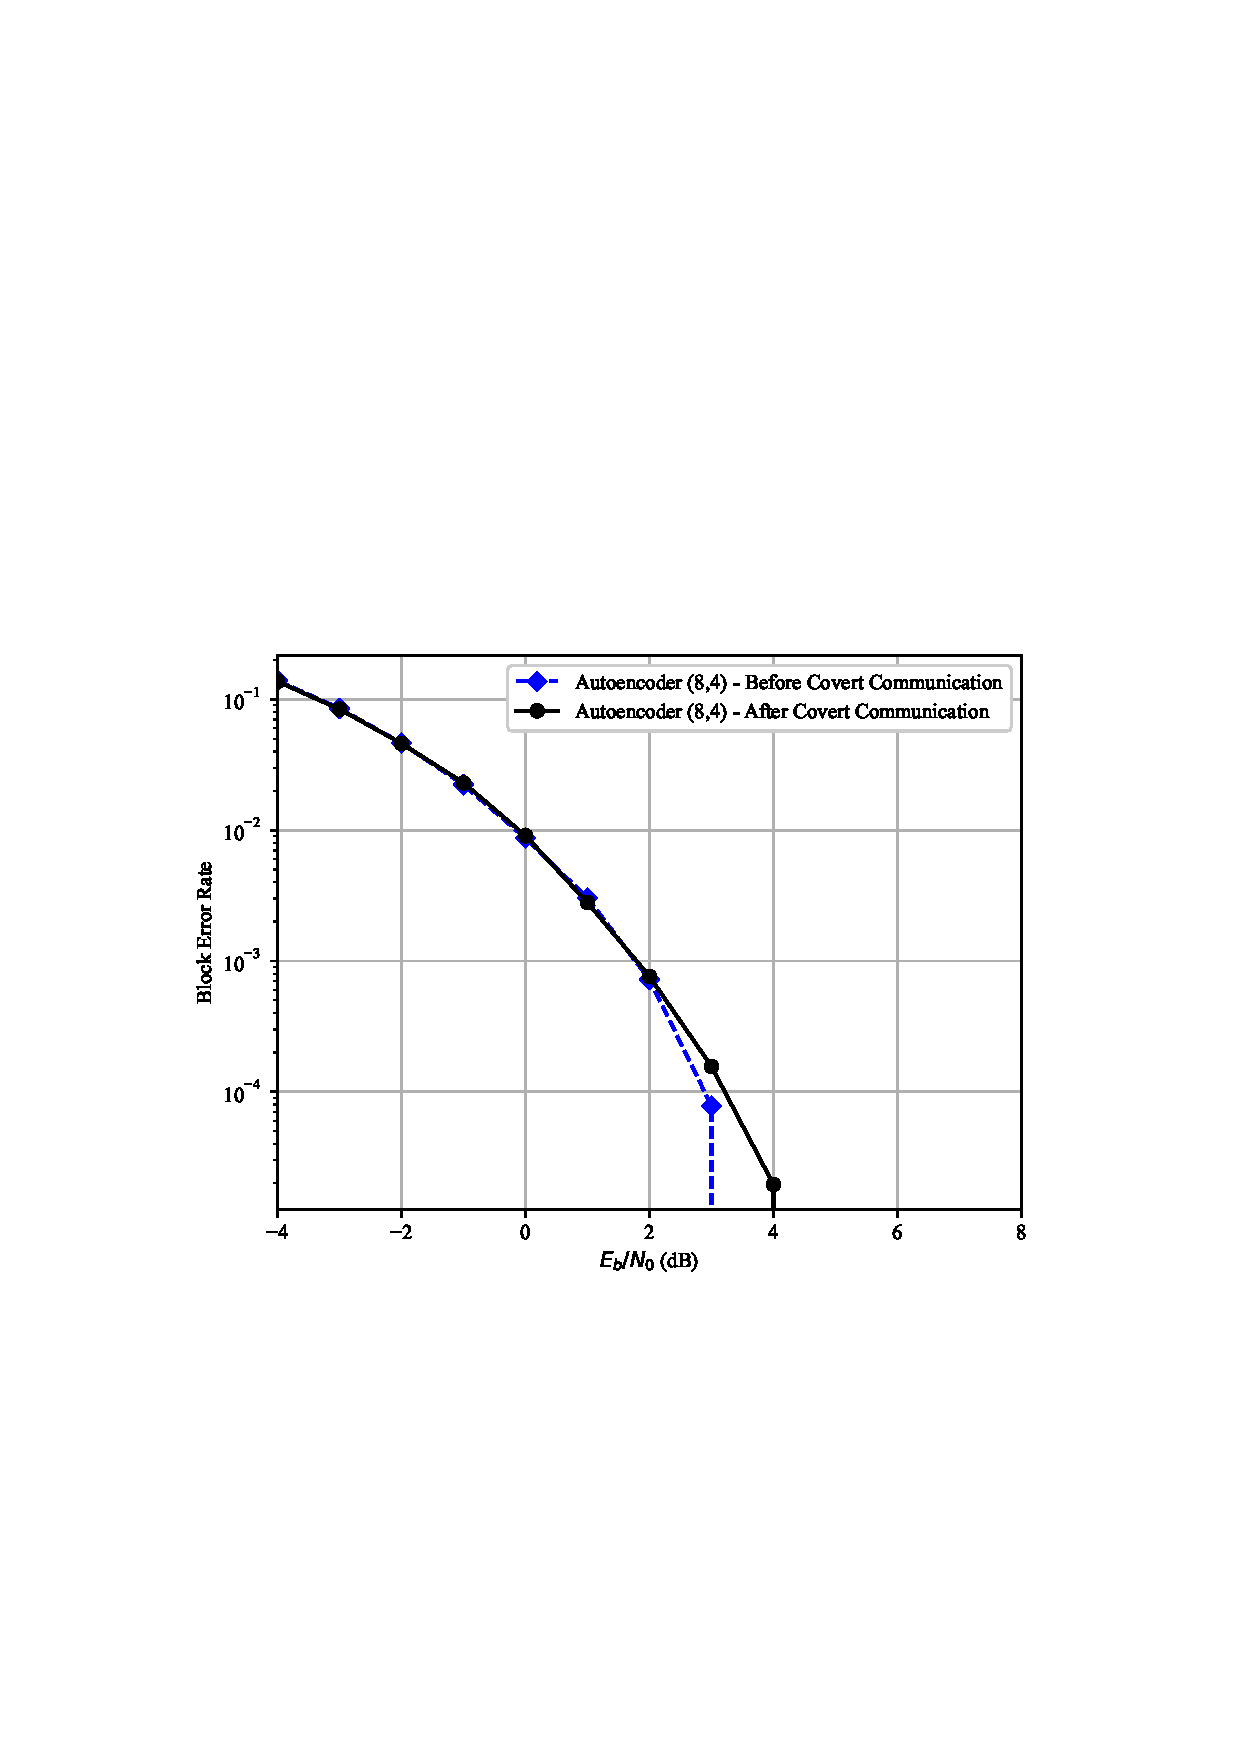
\includegraphics[width=\linewidth]{figs/covert_autoencoder_bler_awgn}
		\caption{User's BLER}
		\label{fig:awgn_resutls_ae}
	\end{subfigure}
	\hspace*{\fill}
	\begin{subfigure}{0.28\textwidth}
		\includegraphics[width=\linewidth]{figs/bob_bler_awgn}
		\caption{Bob's BLER}	
		\label{fig:awgn_resutls_bob}
	\end{subfigure}
	\hspace*{\fill}
	\begin{subfigure}{0.28\textwidth}
		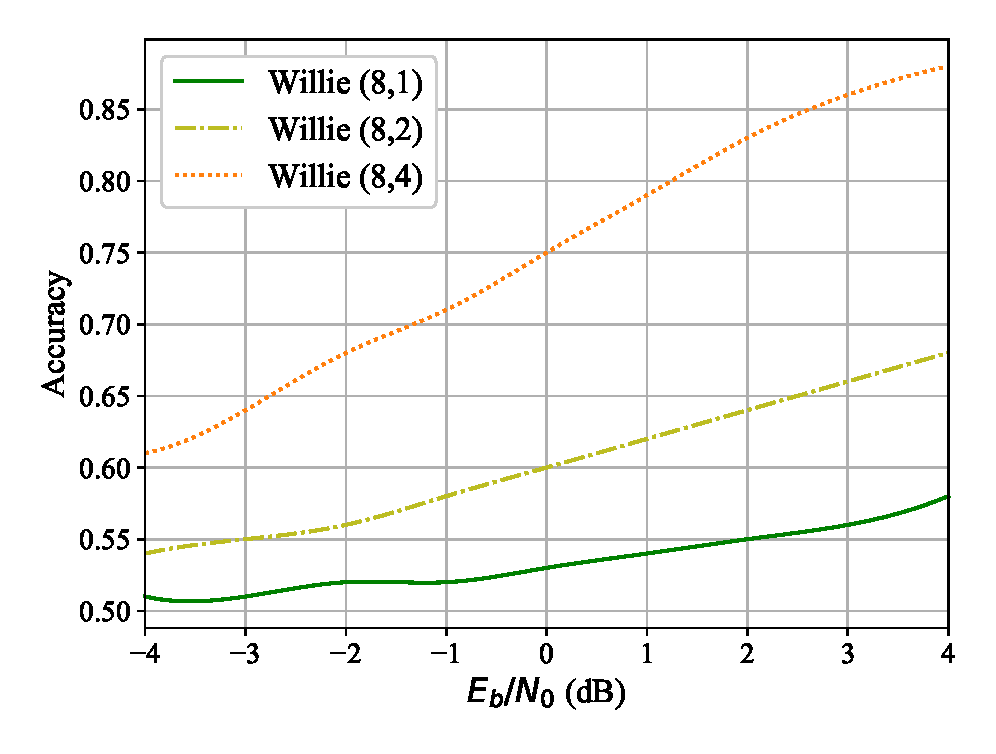
\includegraphics[width=\linewidth]{figs/willie_accuracy_awgn}
		\caption{Willie's accuracy}	
		\label{fig:awgn_resutls_willie}
	\end{subfigure}
	\caption{Single-user covert models' performance over AWGN channel for different covert data rates on a range of SNRs.}
	\label{fig:awgn_results}
\end{figure*}
\begin{figure*}[tp!]
	\begin{subfigure}{0.28\textwidth}
		\includegraphics[width=\linewidth]{figs/covert_autoencoder_bler_rayleigh}
		\caption{User's BLER}
		\label{fig:rayleigh_resutls_ae}
	\end{subfigure}
	\hspace*{\fill}
	\begin{subfigure}{0.28\textwidth}
		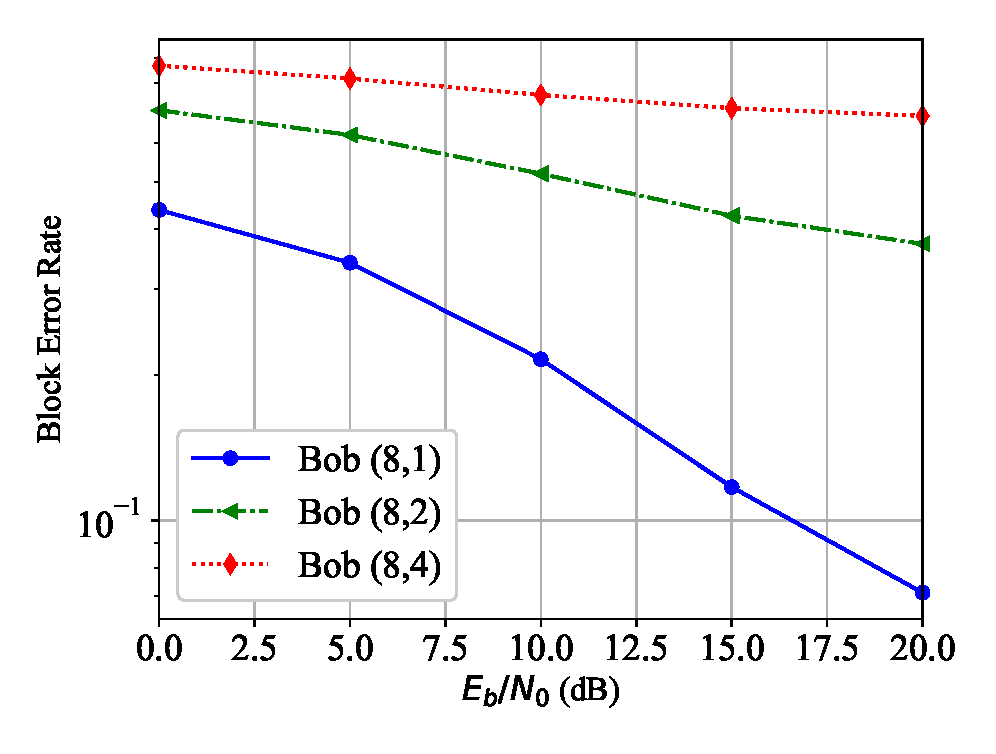
\includegraphics[width=\linewidth]{figs/bob_bler_rayleigh}
		\caption{Bob's BLER}
		\label{fig:rayleigh_resutls_bob}	
	\end{subfigure}
	\hspace*{\fill}
	\begin{subfigure}{0.28\textwidth}
		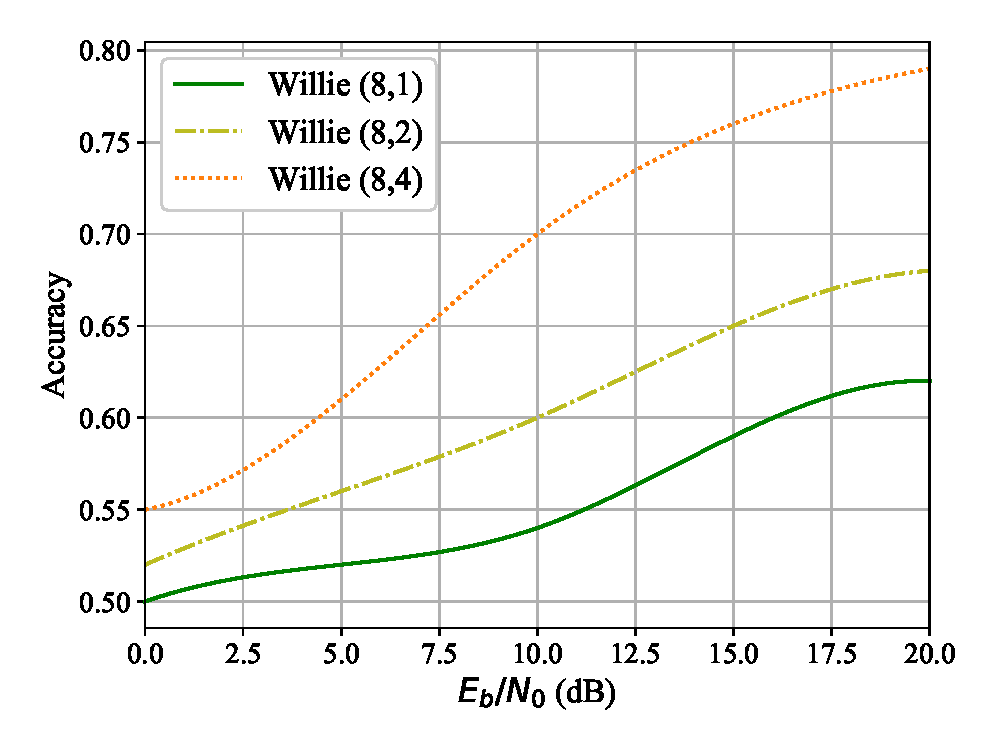
\includegraphics[width=\linewidth]{figs/willie_accuracy_rayleigh}
		\caption{Willie's accuracy}
		\label{fig:rayleigh_resutls_willie}
	\end{subfigure}
	\caption{Single-user covert models' performance over Rayleigh fading channel for different covert data rates on a range of SNRs.}
	\label{fig:rayleigh_resutls}
\end{figure*}
\begin{figure*}[tp!]
	\begin{subfigure}{0.28\textwidth}
		\includegraphics[width=\linewidth]{figs/covert_autoencoder_bler_rician}
		\caption{User's BLER}
		\label{fig:rician_resutls_ae}
	\end{subfigure}
	\hspace*{\fill}
	\begin{subfigure}{0.28\textwidth}
		\includegraphics[width=\linewidth]{figs/bob_bler_rician}
		\caption{Bob's BLER}
		\label{fig:rician_resutls_bob}	
	\end{subfigure}
	\hspace*{\fill}
	\begin{subfigure}{0.28\textwidth}
		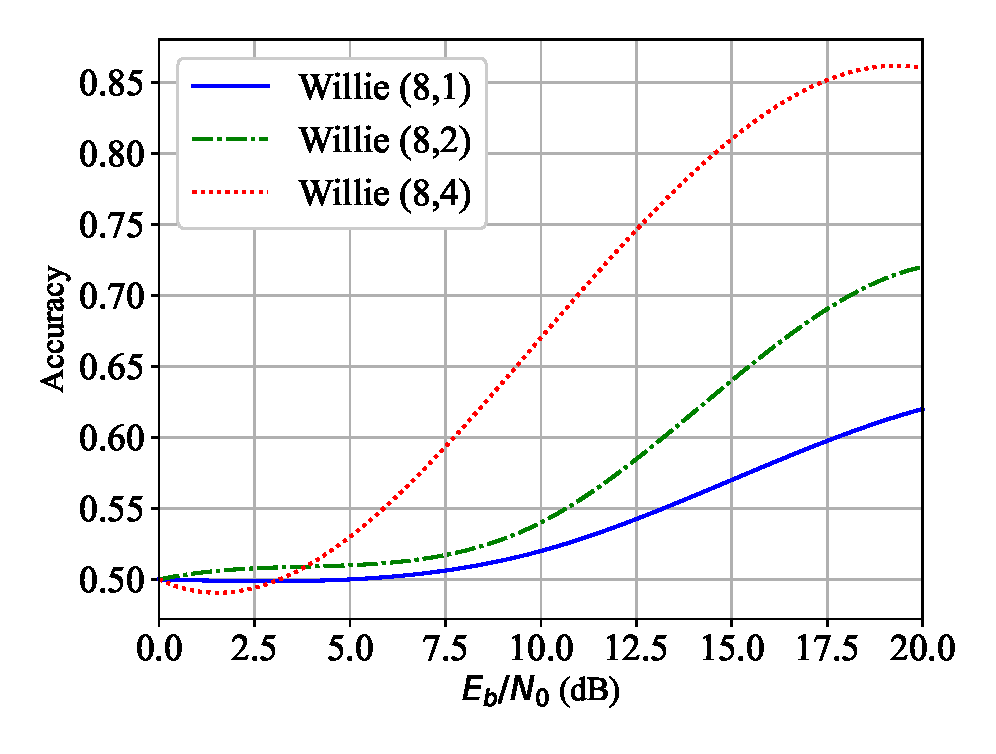
\includegraphics[width=\linewidth]{figs/willie_accuracy_rician}
		\caption{Willie's accuracy}
		\label{fig:rician_resutls_willie}
	\end{subfigure}
	\caption{Single-user covert models' performance over Rician fading channel for different covert data rates on a range of SNRs.}
	\label{fig:rician_resutls}
\end{figure*}


\subsection{Covert Model Performance Evaluation}
We evaluated the performance of our covert communication models on three different channel models: AWGN, Rayleigh fading, and Rician fading. We used the same training procedure for all settings, but the network architecture of our covert and autoencoder models in the multi-user case differed slightly from that in the single-user setting. Table \ref{table:covert_models_structure} shows these differences.

\textbf{Datasets and Hyperparameters}: Since each covert message \(m\) has to be paired with a normal message \(s\), we created the covert model's training and testing sets to have the same number of samples as the autoencoder's. All models were trained for 5000 epochs using the Adam optimizer in an adversarial training setting. We adjusted the importance of each of Alice's objectives by setting \(\lambda_{\mathcal{W}} = 2 \lambda_{\mathcal{B}} = 4 \lambda_{\mathcal{U}}\) for the single-user case, and \(\lambda_{\mathcal{W}} = 3 \lambda_{\mathcal{B}} = 6 \lambda_{\mathcal{U}}\) for the multi-user case in (\ref{alice_loss}). We arrived at these numbers by running a grid search on these parameters. However, our solution is not limited to these parameters, and one can use a different set of parameters to emphasize one specific objective more than the others. In both the single-user and multi-user cases, we started the training with a learning rate of 0.001 for the first 2500 epochs and then made the learning rate ten times smaller for the remaining 2500 epochs. In each epoch, we first updated the parameters of Willie's network using (\ref{willie_loss}), then trained Alice's network for one step using (\ref{alice_loss}), and finally optimized Bob's network based on (\ref{bob_loss}).

\begin{algorithm}[tp!]
	\caption{Optimal SNR range search algorithm}\label{alg:snr_search}
	\small
	\begin{algorithmic}
		\State $acc_{\mathcal{A, B, W}} \gets$ Alice, Bob, and Willie final training accuracies
		\State $p, c \gets$ Previous and current average training accuracies
		\State $snr_{L, U} \gets$ Optimal lower and upper bounds of the SNR range
		\State $t \gets L$ Tracking the SNR bound that is expanding
		\While{true}
		\State $acc_{\mathcal{A}}, acc_{\mathcal{B}}, acc_{\mathcal{W}} \gets Train(snr_{L}, snr_{U})$
		\State $c \gets Avg(acc_{\mathcal{A}}, acc_{\mathcal{B}}, acc_{\mathcal{W}})$
		\If {$c > p$}
		\State $p \gets c$
		\State $snr_{t} \gets snr_{t} \pm 1$
		\Else
		\If {$t$ is equal $L$}
		\State $t \gets U$
		\Else
		\State \Return $snr_{L, U}$
		\EndIf
		\EndIf
		\EndWhile
	\end{algorithmic}
\end{algorithm}

Although we trained our autoencoder network on a fixed SNR value, we found that our covert scheme performed better when trained on a range of SNR values. We achieved this by randomly switching the SNR value within a predetermined range after each epoch of training. Training our models this way not only helped Alice better preserve the normal communication's accuracy but also enabled Bob to decode covert messages more accurately on lower SNR values. Accordingly, we started by setting the training SNR to the value that the autoencoder was trained on and incrementally expanded the SNR range from both ends until no further improvement was observed. Algorithm \ref{alg:snr_search} shows the steps of this process. As a result, in the single-user case, we settled on the range of -2dB to 8 dB for the AWGN channel and 10dB to 30dB for both the Rayleigh and Rician fading channels. In the multi-user system, the optimal range was found within the 0dB to 10dB range for the AWGN channel, 0dB to 20dB for the Rician channel, and 10dB to 30dB for the Rayleigh channel.

\textbf{Training Procedure}: Fig. \ref{fig:traning_progress} shows the progress of each covert actor's accuracy on the test set during the training process for both single-user and multi-user cases. As the training progresses, Bob gradually learns to decode covert messages \(m\) and establishes reliable communication with Alice. After a few epochs as the covert communication begins to take form and stabilize, the signals start to deviate from their original distribution, which helps Willie to better detect covert signals. When Willie's accuracy increases, the term \(\mathcal{L}_{\mathcal{W}}\) dominates the other two objectives of Alice's loss function in (\ref{alice_loss}). As a result, Alice gradually sacrifices accuracy for undetectability. Soon after, the training process reaches a stable point where neither of the covert models sees any significant improvement in accuracy as the training progresses. At the end of the training, the Users' accuracy remains intact, Bob achieves reliable covert communication accuracy, and Willie stabilizes at around 50$\sim$60\% accuracy, which, for a binary classifier, is very close to random guessing accuracy.

\begin{figure*}[tp!]
	\begin{subfigure}{0.28\textwidth}
		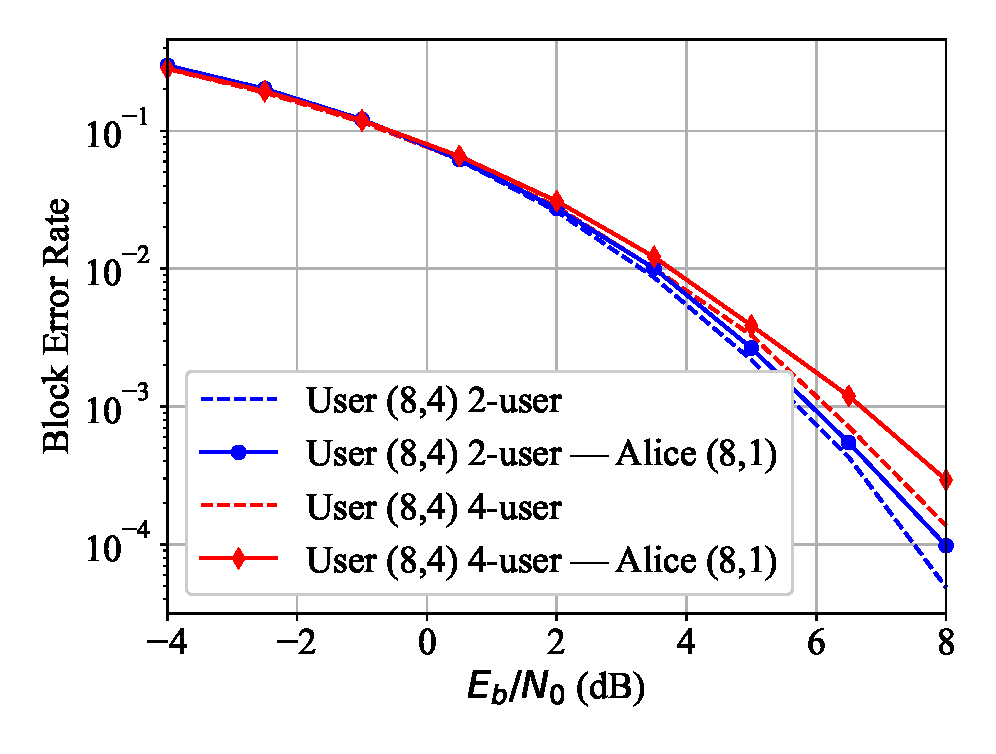
\includegraphics[width=\linewidth]{figs/multi_covert_autoencoder_bler_awgn}
		\caption{User's BLER}
		\label{fig:multi_awgn_results_ae}
	\end{subfigure}
	\hspace*{\fill}
	\begin{subfigure}{0.28\textwidth}
		\includegraphics[width=\linewidth]{figs/multi_bob_bler_awgn}
		\caption{Bob's BLER}	
		\label{fig:multi_awgn_results_bob}
	\end{subfigure}
	\hspace*{\fill}
	\begin{subfigure}{0.28\textwidth}
		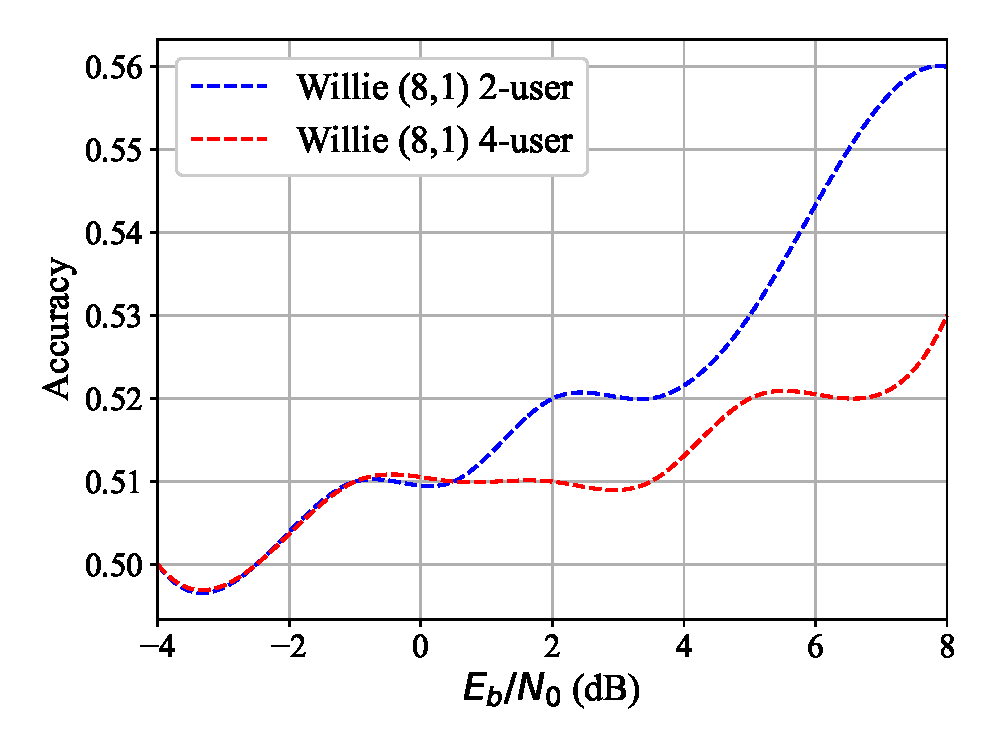
\includegraphics[width=\linewidth]{figs/multi_willie_accuracy_awgn}
		\caption{Willie's accuracy}	
		\label{fig:multi_awgn_results_willie}
	\end{subfigure}
	\caption{Multi-user covert models' performances over AWGN channel for systems with different numbers of users over a range of SNRs.}
	\label{fig:multi_awgn_results}
\end{figure*}
\begin{figure*}[tp!]
	\begin{subfigure}{0.28\textwidth}
		\includegraphics[width=\linewidth]{figs/multi_covert_autoencoder_bler_rayleigh}
		\caption{User's BLER}
		\label{fig:multi_rayleigh_results_ae}
	\end{subfigure}
	\hspace*{\fill}
	\begin{subfigure}{0.28\textwidth}
		\includegraphics[width=\linewidth]{figs/multi_bob_bler_rayleigh}
		\caption{Bob's BLER}
		\label{fig:multi_rayleigh_results_bob}	
	\end{subfigure}
	\hspace*{\fill}
	\begin{subfigure}{0.28\textwidth}
		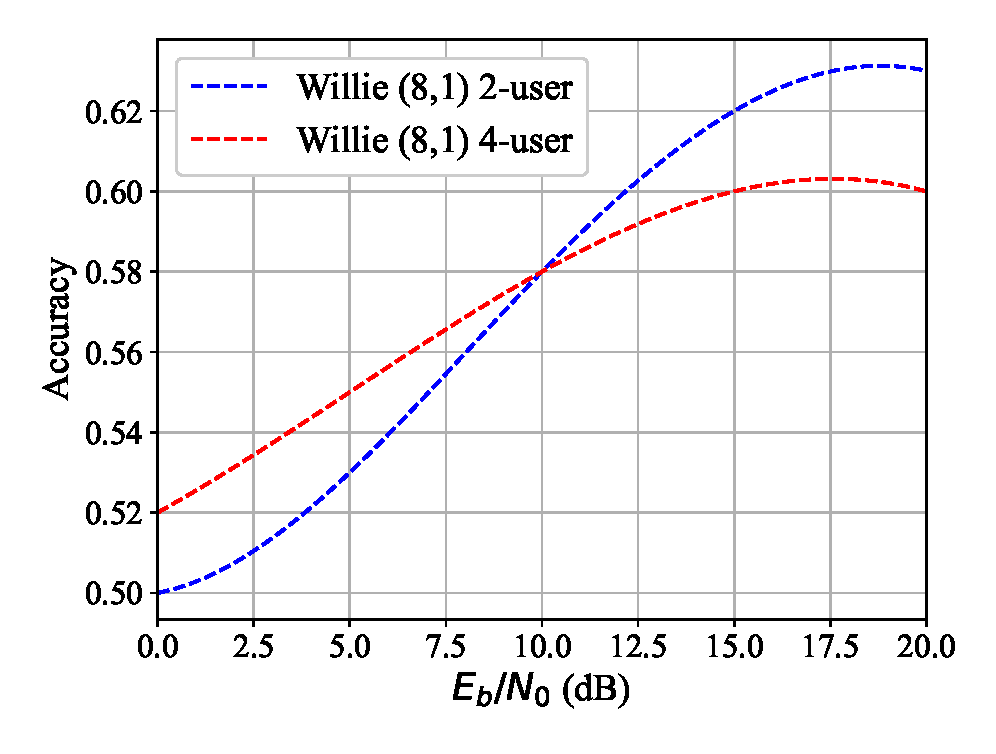
\includegraphics[width=\linewidth]{figs/multi_willie_accuracy_rayleigh}
		\caption{Willie's accuracy}
		\label{fig:multi_rayleigh_results_willie}
	\end{subfigure}
	\caption{Multi-user covert models' performances over Rayleigh channel for systems with different number of users over a range of SNRs.}
	\label{fig:multi_rayleigh_results}
\end{figure*}
\begin{figure*}[tp!]
	\begin{subfigure}{0.28\textwidth}
		\includegraphics[width=\linewidth]{figs/multi_covert_autoencoder_bler_rician}
		\caption{User's BLER}
		\label{fig:multi_rician_results_ae}
	\end{subfigure}
	\hspace*{\fill}
	\begin{subfigure}{0.28\textwidth}
		\includegraphics[width=\linewidth]{figs/multi_bob_bler_rician}
		\caption{Bob's BLER}
		\label{fig:multi_rician_results_bob}	
	\end{subfigure}
	\hspace*{\fill}
	\begin{subfigure}{0.28\textwidth}
		\includegraphics[width=\linewidth]{figs/multi_willie_accuracy_rician}
		\caption{Willie's accuracy}
		\label{fig:multi_rician_results_willie}
	\end{subfigure}
	\caption{Multi-user covert models' performances over Rician channel for systems with different number of users over a range of SNRs.}
	\label{fig:multi_rician_results}
\end{figure*}

\textbf{Single-User Experiments}: 
We started our experiments with the single-user case. First, we evaluated our covert models by sending 1 bit of covert data over 8 channel uses and then gradually increased the number of covert bits to see how increasing the covert data rate affected each component of our covert scheme. We used the notations \(Alice (n,k)\), \(Bob (n,k)\), and \(Willlie (n,k)\) to differentiate models with different covert data rates, and their interpretation was the same as that of the autoencoder model.

Figures \ref{fig:awgn_results}, \ref{fig:rayleigh_resutls}, and \ref{fig:rician_resutls} illustrate the performance of our scheme for different covert data rates and how reliable our covert models are at different covert data rates. As we expected, with increasing covert data rates, covert communication becomes more unreliable, its impact on the normal communication increases, and detection becomes easier for Willie. Overall, these plots indicate that sending covert data at high rates makes covert communication unreliable.

The plots also reveal how the communication channel affects the performance of each actor. In the AWGN channel, higher covert rates have a relatively smaller impact on the User's BLER, while in the fading channels, their impact is more significant. On the other hand, increasing the covert rate in the fading channels has less effect on the covert communication accuracy compared to the AWGN channel. For Willie, all channels exhibit a similar trend, where higher covert rates are more susceptible to detection.

Through these experiments, we have concluded that the most reliable covert data rate is achieved by sending 1 bit of data over 8 channel uses. Therefore, we will be using these parameters as the default when evaluating our models in the multi-user scenario.

\textbf{Multi-User Experiments}: 
After evaluating the reliability of our covert models for different covert data rates, we now aim to measure the robustness of our covert scheme against the number of users in the multi-user scenario. To do this, we evaluate our covert models in systems comprising of 2 and 4 users. This will help us understand how adding users, i.e., increasing interference, affects  the performance of our covert models, and whether it has a more significant impact on communication than increasing the covert data rate.

Figures \ref{fig:multi_awgn_results}, \ref{fig:multi_rayleigh_results}, and \ref{fig:multi_rician_results} present our results for 2-user and 4-user systems, demonstrating how the number of users in the system affects our model's performance. For the AWGN channel, we observe that adding more users does not change the model's overall performance. Furthermore, as the number of users increases, there is almost no impact on the normal receivers from the covert transmissions, and Bob and Willie's performances remain almost the same.

\begin{figure*}[tp!]
	\center
	\begin{subfigure}{0.325\linewidth}
		\begin{subfigure}{0.48\textwidth}
			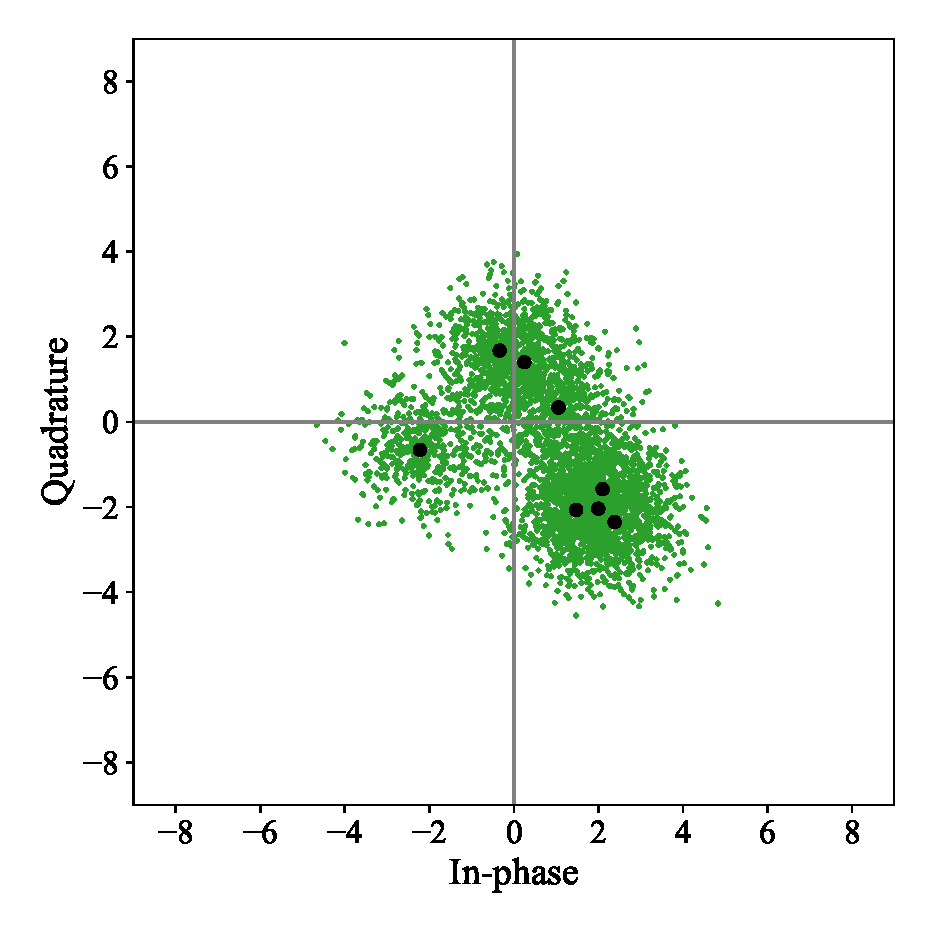
\includegraphics[width=\linewidth]{figs/awgn_normal_constellation}
		\end{subfigure}
		\hfill
		\begin{subfigure}{0.48\textwidth}
			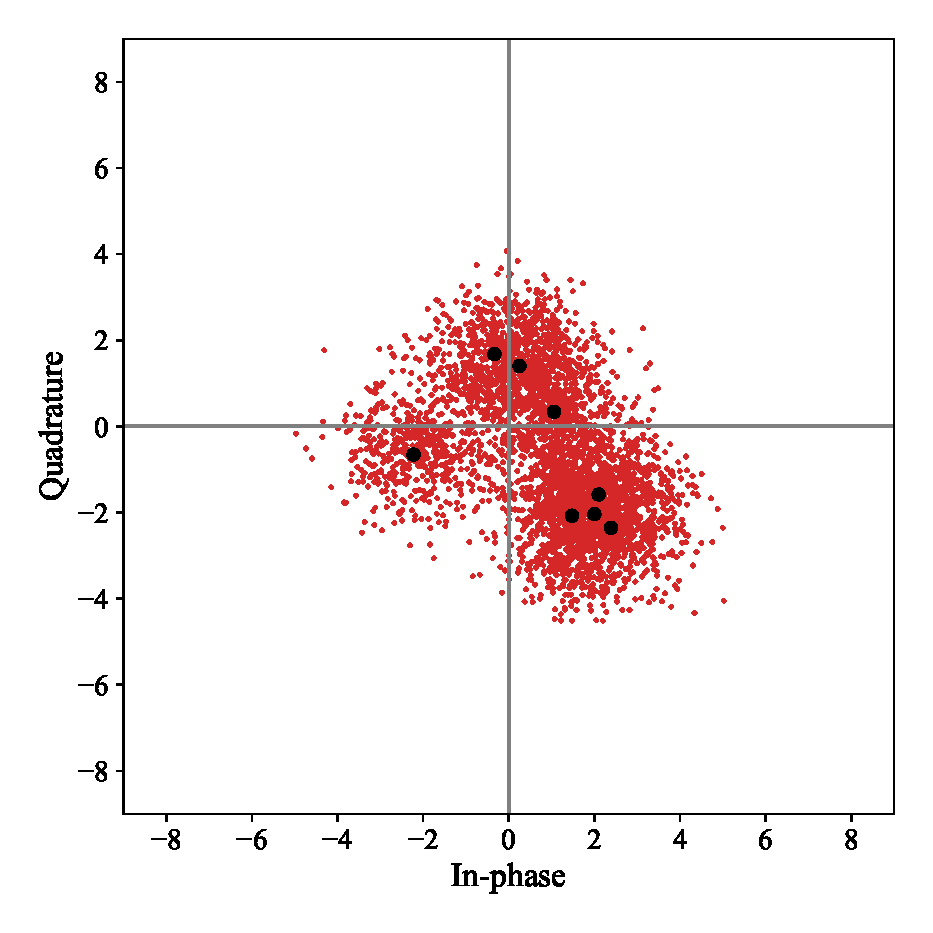
\includegraphics[width=\linewidth]{figs/awgn_covert_constellation}
		\end{subfigure}
		\caption{AWGN channel constellations.}
		\label{fig:awgn_constellation}
	\end{subfigure}
	\begin{subfigure}{0.325\linewidth}
		\begin{subfigure}{0.48\textwidth}
			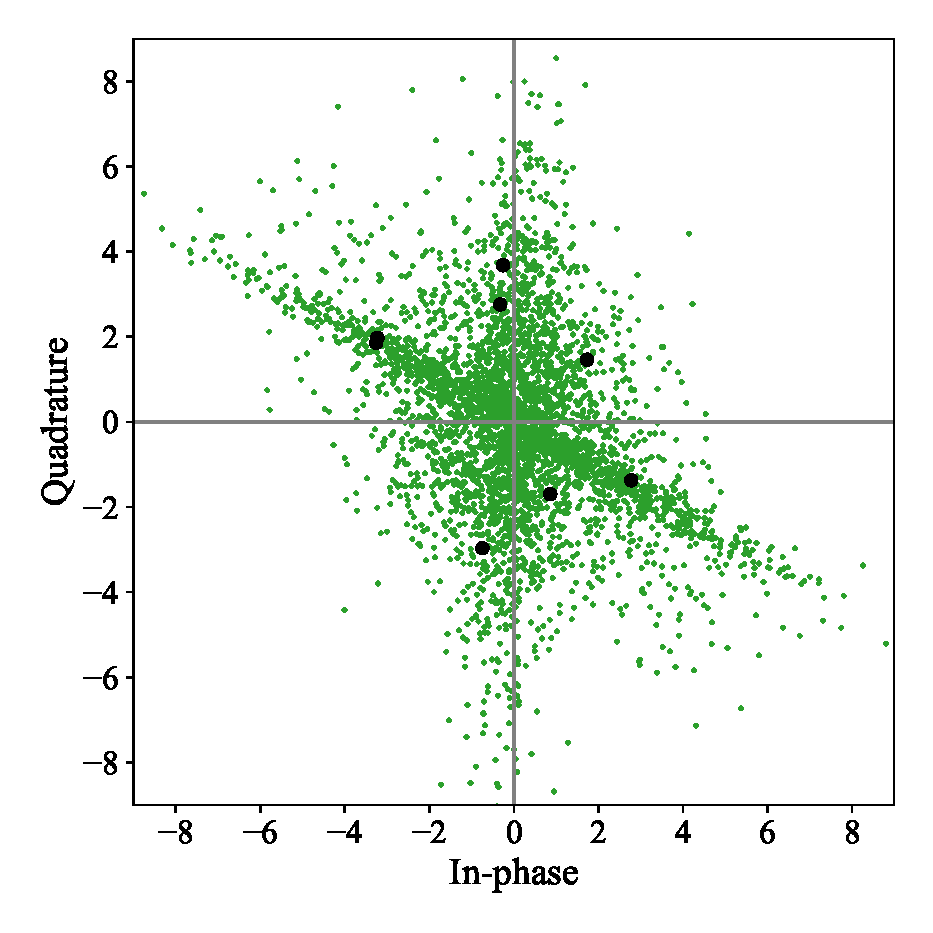
\includegraphics[width=\linewidth]{figs/rayleigh_normal_constellation}
		\end{subfigure}
		\hfill
		\begin{subfigure}{0.48\textwidth}
			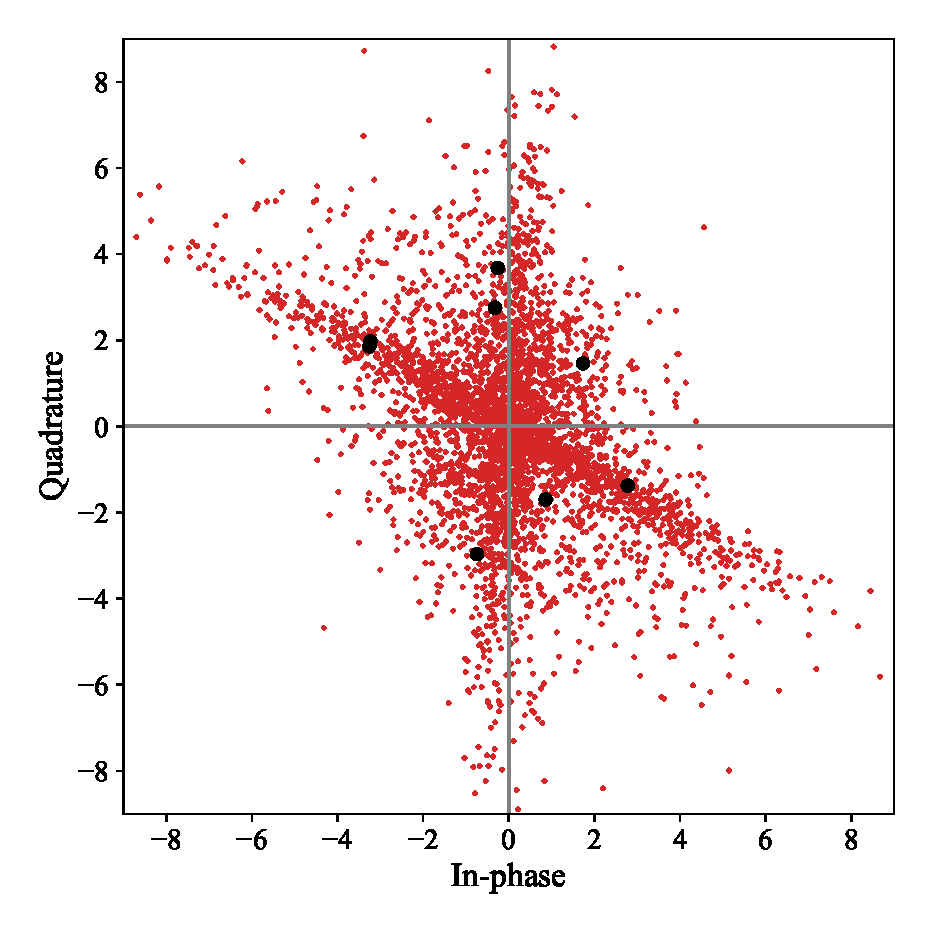
\includegraphics[width=\linewidth]{figs/rayleigh_covert_constellation}
		\end{subfigure}
		\caption{Rayleigh fading channel constellations}
		\label{fig:rayleigh_constellation}
	\end{subfigure}
	\begin{subfigure}{0.325\linewidth}
		\begin{subfigure}{0.48\textwidth}
			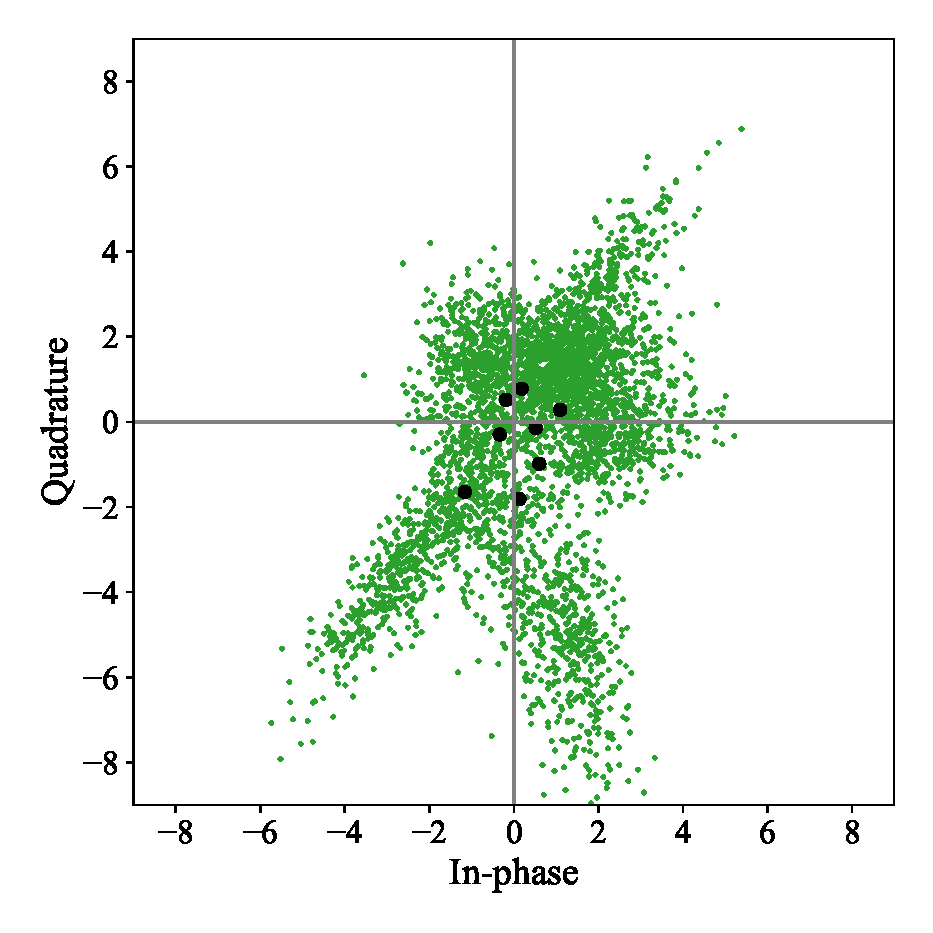
\includegraphics[width=\linewidth]{figs/rician_normal_constellation}
		\end{subfigure}
		\hfill
		\begin{subfigure}{0.48\textwidth}
			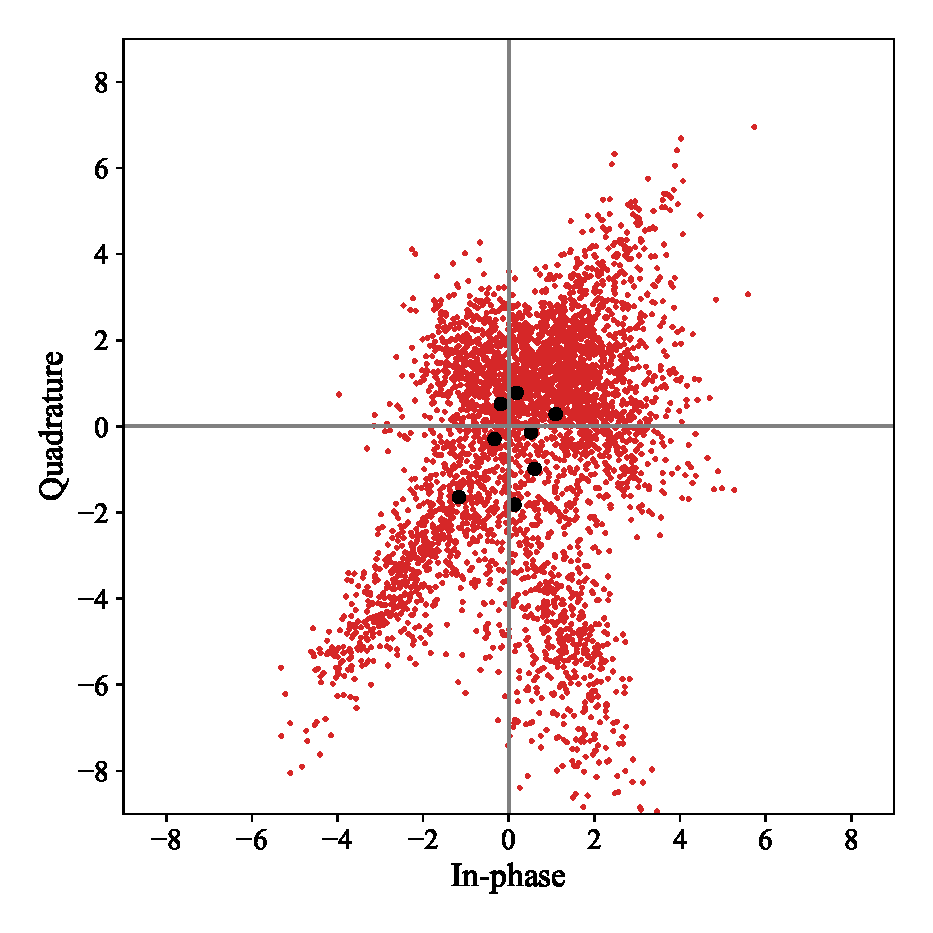
\includegraphics[width=\linewidth]{figs/rician_covert_constellation}
		\end{subfigure}
		\caption{Rician fading channel constellations}
		\label{fig:rician_constellation}
	\end{subfigure}
	\caption{Comparing AWGN, Rayleigh and Rician fading channels constellation clouds of a sample signal. The green clouds show the constellation before the covert communication and the red clouds show it after.}
\end{figure*}


However, for the Rayleigh and Rician channels, a degree of freedom effect can be noticed, where increasing number of users makes it more challenging for the covert users to avoid interfering with the ongoing normal communication. As a result, the impact of covert communication on normal users becomes more detrimental with a higher number of users. Unlike in the AWGN channel, adding more users in these cases significantly affects Bob's performance, rendering covert communication practically ineffective. Looking at Figs. \ref{fig:multi_rayleigh_results} and \ref{fig:multi_rician_results}, we can observe a distinct cross-over pattern for the fading channels. Specifically, Figs. \ref{fig:multi_rayleigh_results_ae} and \ref{fig:multi_rician_results_ae} reveal that there is a certain SNR at which the covert communication in the 4-user systems begins to have a greater impact on normal communication compared to the 2-user systems. These SNRs are 5dB, 10db in the Rayleigh and Rician channels, respectively. These points indicate that covert users can no longer communicate reliably without causing interference to normal users. This behavior is even more apparent in Figs. \ref{fig:multi_rayleigh_results_bob} and \ref{fig:multi_rician_results_bob}, which show that Bob's BLER begins to degrade at the same SNR values and eventually plateaus, deviating from the performance of the 2-user system. Likewise, we can see the same pattern in Willie's detection accuracy. Since covert communication has no specific pattern from these points further,Willie is unable to detect it accurately and thereby his detection accuracy remains constant.

\textbf{Undetectability}: Willie's detection accuracy can be found in figs. \ref{fig:awgn_resutls_willie}, \ref{fig:rayleigh_resutls_willie}, and \ref{fig:rician_resutls_willie} for the single-user case, and in Figures \ref{fig:multi_awgn_results_willie}, \ref{fig:multi_rayleigh_results_willie}, \ref{fig:multi_rician_results_willie} for the multi-user case. His detection performance is evaluated over a range of SNR values for detecting signals as covert and normal. In the single-user experiments, we observe that as the covert data rate increases, the covert communication becomes more easily detectable. In the multi-user case, we cannot directly compare Willie's accuracy for different numbers of users because covert users are unable to establish their covert communication in the fading channels in systems with 4 users. However, the results from the AWGN channel indicate that Willie's accuracy remains roughly the same as we increase the number of users.

\textbf{Constellation Diagrams}: Figs. \ref{fig:awgn_constellation}, \ref{fig:rayleigh_constellation}, and \ref{fig:rician_constellation} compare the constellation clouds of covert and normal signals for AWGN, Rayleigh, and Rician fading channels in the single-user system. We marked each symbol of the encoder's output signal as black circle points on the constellation diagrams. The red constellation cloud shows how covert signals scatter after passing through the channel, and the green cloud shows this for normal signals. Since data is sent over 8 channel uses, there are 8 black points on the chart. To maintain consistency with Willie's accuracy and Bob's error rate for all channel models, we set the SNR value to 6dB for the AWGN, 15dB for the Rayleigh fading channel, and 16dB for the Rician fading channel. This ensured that, in all channel models, the probability of detection remained relatively the same, and the covert communication BLER stayed below \(10^{-1}\). This area of operation provided Alice and Bob relative reliability in their covert communication while maintaining their covertness.
Looking at these figures, the signal constellation diagrams before and after applying our covert model are very similar, showing that Alice has perfectly learned to cloak the covert signals into the distribution of the channel's noise.
\section{Conclusion}

\label{s:conc}


\bibliographystyle{IEEEtran}
% argument is your BibTeX string definitions and bibliography database(s)
\bibliography{bib/main}

% biography section
% 
% If you have an EPS/PDF photo (graphicx package needed) extra braces are
% needed around the contents of the optional argument to biography to prevent
% the LaTeX parser from getting confused when it sees the complicated
% \includegraphics command within an optional argument. (You could create
% your own custom macro containing the \includegraphics command to make things
% simpler here.)
%\begin{IEEEbiography}[{\includegraphics[width=1in,height=1.25in,clip,keepaspectratio]{mshell}}]{Michael Shell}
% or if you just want to reserve a space for a photo:
\begin{IEEEbiography}[{
		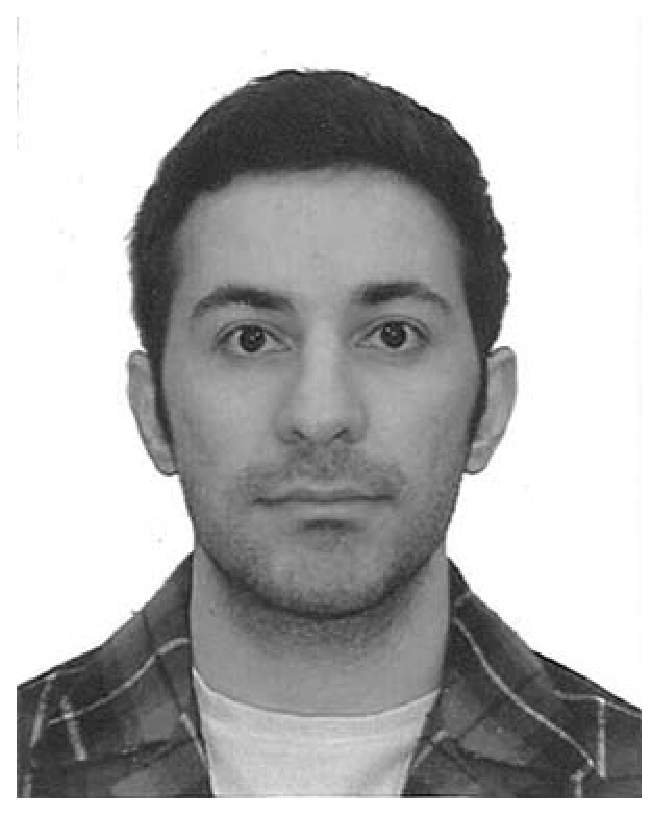
\includegraphics[width=1in,height=1.25in,clip,keepaspectratio]{figs/mohammadi.eps}
	}]{Ali Mohammadi Teshnizi}
	(Student Member, IEEE) received the B.S. degree in computer engineering from
	University of Tehran in 2020. He is currently pursuing the M.S. degree in computer science with University of Calgary, where he is a Research
	Assistant. His research interests include the applications of machine learning and deep learning, radio communications and network security, and the Internet of Things (IoT).
\end{IEEEbiography}
\vskip-1.5 \baselineskip
\begin{IEEEbiography}
	[{
	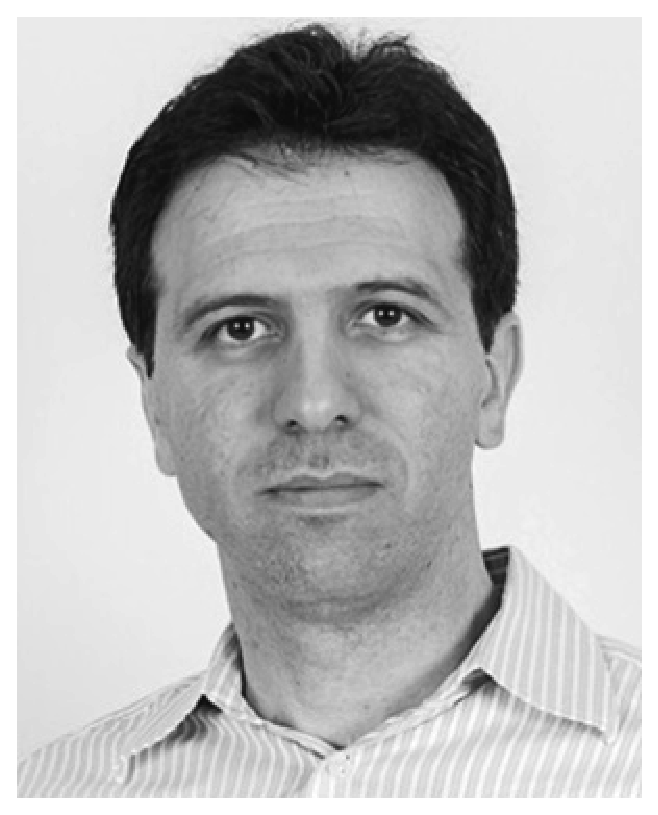
\includegraphics[width=1in,height=1.25in,clip,keepaspectratio]{figs/ghaderi.eps}
	}]{Majid Ghaderi}
(Member, IEEE) received the B.Sc. and M.Sc. degrees in computer science from the Sharif University of Technology and the Ph.D. degree in computer science from the University of Waterloo. He is a Professor with the Computer Science Department, University of Calgary. His general area of research is computer networks. In the broader context of computer networks, his current research focus is on: design and optimization of network algorithms, secure communication in networked systems, and Application of machine learning in network control. The unifying theme of his research is the fusion of theoretical research with real-world applications in the computer networking area.
\end{IEEEbiography}
\vskip-2.5\baselineskip
\begin{IEEEbiography}[{
		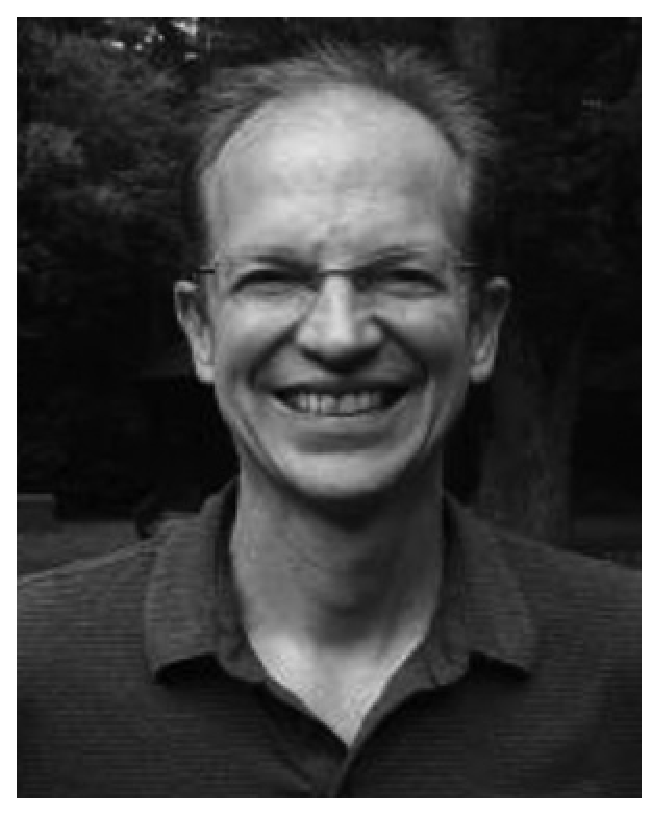
\includegraphics[width=1in,height=1.25in,clip,keepaspectratio]{figs/goeckel.eps}
	}]{Dennis Goeckel}
(Fellow, IEEE) received the B.S. degree from Purdue University, West Lafayette, IN, USA, in 1992, and the M.S. and Ph.D. degrees from the University of Michigan, Ann Arbor, MI, USA, in 1993 and 1996, respectively.,Since 1996, he has been with the ECE Department, University of Massachusetts at Amherst, Amherst, MA, USA, where he is currently a Professor. Prof. Goeckel received the University of Massachusetts Distinguished Teaching Award in 2007. He received the NSF CAREER Award in 1999 and is an IEEE Fellow for ``contributions to wireless communication systems and networks''. He was a Lilly Teaching Fellow from 2000 to 2001.
\end{IEEEbiography}

% if you will not have a photo at all:
%\begin{IEEEbiographynophoto}{John Doe}
%	Biography text here.
%\end{IEEEbiographynophoto}

% insert where needed to balance the two columns on the last page with
% biographies
%\newpage

%\begin{IEEEbiographynophoto}{Jane Doe}
%	Biography text here.
%\end{IEEEbiographynophoto}

% You can push biographies down or up by placing
% a \vfill before or after them. The appropriate
% use of \vfill depends on what kind of text is
% on the last page and whether or not the columns
% are being equalized.

%\vfill

% Can be used to pull up biographies so that the bottom of the last one
% is flush with the other column.
%\enlargethispage{-1in}

\vfill

% if have a single appendix:
%\appendix[Proof of the Zonklar Equations]
% or
%\appendix  % for no appendix heading
% do not use \section anymore after \appendix, only \section*
% is possibly needed

% use appendices with more than one appendix
% then use \section to start each appendix
% you must declare a \section before using any
% \subsection or using \label (\appendices by itself
% starts a section numbered zero.)
%


\appendix[Model Parameters]

%Table \ref{table:autoencoder_structure} presents the layer configuration and output sizes %of the autoencoder DNN models used in the single-user and multi-user case. Table %\ref{table:covert_models_structure} displays the DNN model structure of the covert actors %and their differences in single-user and multi-user case.

\begin{table*}[!th]
		\caption{Autoencoder's detailed network architecture in the single-user and multi-user case.}
	\begin{adjustbox}{width=1\textwidth,center}
		\begin{tabular}{c|c|c|c|c|c|}
			\cline{2-6}
			& \textbf{UserTX Encoder} & \textbf{UserRX Parameter Estimation} & \textbf{UserRX Decoder} & \textbf{BaseRX  Pre-Decoder} & \textbf{BaseRX Decoders} \\ \hline
			\multicolumn{1}{|c|}{input size} & 16 & 2 $\times$ 16 & 2 $\times$ 8 & $n_{tx} \times$ 2 $\times$ 8 & $n_{tx} \times$ 4 $\times$ 8 \\ \hline
			\multicolumn{1}{|c|}{dense layers sizes} & 2 $\times$ 8, 2 $\times$ 8 & 2 $\times$ 16, 2 $\times$ 32, 2 $\times$ 8 & 2 $\times$ 8, 2 $\times$ 8 & \begin{tabular}[c]{@{}c@{}}$n_{tx} \times$ 2 $\times$ 8, $n_{tx} \times$ 4 $\times$ 8\end{tabular} & $n_{tx} \times$ 2 $\times$ 8 \\ \hline
			\multicolumn{1}{|c|}{dense layers activations} & 2 $\times$ ELU & ELU, 2 $\times$ Tanh & 2 $\times$ Tanh, Softmax & 3 $\times$ Tanh & Tanh, Softmax \\ \hline
			\multicolumn{1}{|c|}{conv filters} & 1, 8, 8, 8 & - & 1, 8, 8, 8 & 1, 8, 8, 8 & - \\ \hline
			\multicolumn{1}{|c|}{conv kernel sizes} & 2, 4, 2, 2 & - & 2, 4, 2, 2 & 2, 4, 2, 2 & - \\ \hline
			\multicolumn{1}{|c|}{conv strides} & 1, 2, 1, 1 & - & 1, 2, 1, 1 & 1, 2, 1, 1 & - \\ \hline
			\multicolumn{1}{|c|}{conv activations} & 4 $\times$ Tanh & - & 4 $\times$ Tanh & 4 $\times$ Tanh & - \\ \hline
			\multicolumn{1}{|c|}{output size} & 2 $\times$ 8 & 2 $\times$ 1 & 16 & $n_{tx} \times$ 4 $\times$ 8 & 16 \\ \hline
		\end{tabular}
	\end{adjustbox}
	\label{table:autoencoder_structure}
\end{table*}

\begin{table}[!th]
		\caption{Alice, Bob, and Willie's detailed network architecture in the single-user and multi-user case.}
	\begin{adjustbox}{width=1\textwidth,center}
		\begin{tabular}{c|c|c|c|c|c|}
			\cline{2-6}
			\multicolumn{1}{l|}{} & \textbf{Alice (Single-User)} & \textbf{Alice (Multi-User) AWGN} & \textbf{Alice (Multi-User) Rayleigh/Rician} & \textbf{Bob} & \textbf{Willie} \\ \hline
			\multicolumn{1}{|c|}{input size} & 16 + $2^{k}$ & 16  + $2^{k}$ & 16  + $2^{k+1}$ + ($n_{tx} \times n_{tx} \times 2$) & 16 & 16 \\ \hline
			\multicolumn{1}{|c|}{dense layers sizes} & \begin{tabular}[c]{@{}c@{}}32  + $2^{k+1}$, \\ 32 + $2^{k+1}$, \\ 8 $\times 2^k$\end{tabular} & \begin{tabular}[c]{@{}c@{}}32  + $2^{k+1}$, \\ 32 + $2^{k+1}$, \\ 8 $\times 2^k$\end{tabular} & \begin{tabular}[c]{@{}c@{}}32  + $2^{k+1}$ + ($n_{tx} \times n_{tx} \times 2$),\\ 32 + $2^{k+1}$, \\ 32 + $2^{k+1}$, \\ 8 $\times 2^k$\end{tabular} & 2 $\times$ 8, 16 & 2 $\times$ 8, 2 $\times$ 8 \\ \hline
			\multicolumn{1}{|c|}{dense layers activations} & 3 $\times$ ReLU, Tanh & 3 $\times$ ReLU, Tanh & 4 $\times$ ReLU, Tanh & 2 $\times$ Tanh, Softmax & 2 $\times$ Tanh, Sigmoid \\ \hline
			\multicolumn{1}{|c|}{conv filters} & - & - & - & 1, 8, 8, 8, 8 & 1, 8, 8, 8, 8 \\ \hline
			\multicolumn{1}{|c|}{conv kernel sizes} & - & - & - & 1, 2, 4, 2, 2 & 1, 2, 4, 2, 2 \\ \hline
			\multicolumn{1}{|c|}{conv strides} & - & - & - & 1, 1, 2, 1, 1 & 1, 1, 2, 1, 1 \\ \hline
			\multicolumn{1}{|c|}{conv activations} & - & - & - &  5 $\times$ LeakyReLU & 5 $\times$ LeakyReLU \\ \hline
			\multicolumn{1}{|c|}{output size} & 2 $\times$ 8 & 2 $\times$ 8 & 2 $\times$ 8 & $2^{k}$ & 1 \\ \hline
		\end{tabular}
	\end{adjustbox}
	\label{table:covert_models_structure}
\end{table}

\end{document}


